\resizebox {\columnwidth} {!} {
\begin{tikzpicture}

\def\da{2cm}
\def\db{20mm}
\def\dc{6mm}

\node [fill=white] (root) {(1)}
    child [line width=.5pt] { [sibling distance=\db] node [fill=white] (n10) {(10)}
      child {node (n100) {(100)} [sibling distance=\dc]
      	child { node[fill=red,circle,inner sep=1.5pt,draw] (n1000) {} }
      	child { node[fill=blue,circle,inner sep=1.5pt,draw] (n1001) {} }
      	child { node[fill=black!20!green,circle,inner sep=1.5pt,draw] (n1002) {} }
      	child { node[fill=black,circle,inner sep=1.5pt,draw] (n1003) {} }
      }
      child {node (n101) {(101)} [sibling distance=\dc]
      	child { node[fill=black!10,circle,inner sep=1.5pt,draw] (n1010) {} }
      }
      child {node (n102) {(102)} [sibling distance=\dc]
      	child { node[fill=orange,circle,inner sep=1.5pt,draw] (n1020) {} }
      	child { node[] (n1021) {$\times$} }
      	child { node[] (n1022) {$\times$} }
      }
      child {node {(103)} [sibling distance=\dc]
      }
    }
    child [line width=.5pt,dashed] { node [fill=white] {(11)}
    }
    child [line width=.5pt,dashed] { node [fill=white] {(12)}
    }
    child [line width=.5pt,dashed] { node [fill=white] {(13)}
    }
;
%\draw[dashed,<->,red] ([yshift=-4pt]n1000.south east) to [out=-30,in=210] ([yshift=-4pt]n1001.south west);
%\draw[dashed,<->,red] ([yshift=-4pt]n1000.south east) to [out=-30,in=210] ([yshift=-4pt]n1002.south west);
%\draw[dashed,<->,red] ([yshift=-4pt]n1000.south east) to [out=-30,in=210] ([yshift=-4pt]n1003.south west);
\draw[red,->,thick] ([yshift=7pt]root.south west) -- ([yshift=5pt]n10.north east);
\draw[red,->,thick] ([yshift=9pt]n10.south west) -- ([yshift=6pt]n100.north east);
\draw[red,->,thick] ([xshift=6pt]n100.south west) -- ([yshift=2pt,xshift=-6pt]n1000.north east);

\draw[blue,->,thick] ([yshift=12pt]root.south west) -- ([yshift=10pt]n10.north east);
\draw[blue,->,thick] ([yshift=14pt]n10.south west) -- ([yshift=11pt]n100.north east);
\draw[blue,->,thick] ([xshift=12pt]n100.south west) -- ([yshift=2pt,xshift=-5pt]n1001.north east);

\draw[black!20!green,->,thick] ([yshift=17pt]root.south west) -- ([yshift=15pt]n10.north east);
\draw[black!20!green,->,thick] ([yshift=19pt]n10.south west) -- ([yshift=16pt]n100.north east);
\draw[black!20!green,->,thick] ([xshift=16pt]n100.south west) -- ([yshift=2pt,xshift=-5pt]n1002.north east);


\draw[black,->,thick] ([yshift=22pt]root.south west) -- ([yshift=20pt]n10.north east);
\draw[black,->,thick] ([yshift=24pt]n10.south west) -- ([yshift=21pt]n100.north east);
\draw[black,->,thick] ([xshift=26pt]n100.south west) -- ([yshift=2pt,xshift=1pt]n1003.north east);

\draw[red,thick] ([yshift=-3pt]n1000.south) |- ([yshift=-8pt]n1000.south) -- ([yshift=-8pt]n1002.south) -| ([yshift=-3pt]n1002.south);
\draw[blue,thick] ([yshift=-11pt]n1000.south) |- ([yshift=-16pt]n1000.south) -- ([yshift=-16pt]n1003.south) -| ([yshift=-11pt]n1003.south);
\draw[black!20!green,thick] ([yshift=-19pt]n1000.south) |- ([yshift=-24pt]n1000.south) -- ([yshift=-24pt]n1010.south) -| ([yshift=-19pt]n1010.south);
\draw[black,thick] ([yshift=-27pt]n1001.south) |- ([yshift=-32pt]n1001.south) -- ([yshift=-32pt]n1020.south) -| ([yshift=-27pt]n1020.south);

%\end{tikzpicture}
%}
%\resizebox {.45\columnwidth} {!} {
%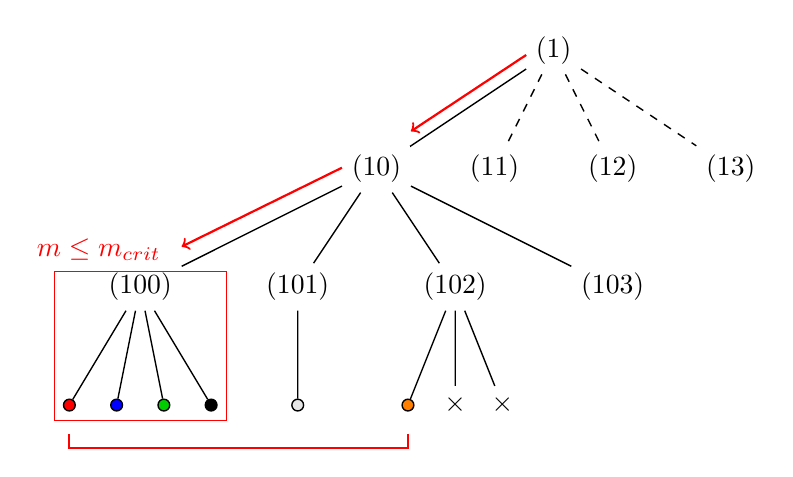
\begin{tikzpicture}

\def\da{2cm}
\def\db{20mm}
\def\dc{6mm}

\node [fill=white] at (9,0) (root) {(1)}
    child [line width=.5pt] { [sibling distance=\db] node [fill=white] (n10) {(10)}
      child {node (n100) {(100)} [sibling distance=\dc]
      	child { node[fill=red,circle,inner sep=1.5pt,draw] (n1000) {} }
      	child { node[fill=blue,circle,inner sep=1.5pt,draw] (n1001) {} }
      	child { node[fill=black!20!green,circle,inner sep=1.5pt,draw] (n1002) {} }
      	child { node[fill=black,circle,inner sep=1.5pt,draw] (n1003) {} }
      }
      child {node {(101)} [sibling distance=\dc]
      	child { node[fill=black!10,circle,inner sep=1.5pt,draw] (n1010) {} }
      }
      child {node {(102)} [sibling distance=\dc]
      	child { node[fill=orange,circle,inner sep=1.5pt,draw] (n1020) {} }
      	child { node[] (n1021) {$\times$} }
      	child { node[] (n1022) {$\times$} }
      }
      child {node {(103)} [sibling distance=\dc]
      }
    }
    child [line width=.5pt,dashed] { node [fill=white] {(11)}
    }
    child [line width=.5pt,dashed] { node [fill=white] {(12)}
    }
    child [line width=.5pt,dashed] { node [fill=white] {(13)}
    }
;
%\draw[dashed,<->,red] ([yshift=-4pt]n1000.south east) to [out=-30,in=210] ([yshift=-4pt]n1001.south west);
%\draw[dashed,<->,red] ([yshift=-4pt]n1000.south east) to [out=-30,in=210] ([yshift=-4pt]n1002.south west);
%\draw[dashed,<->,red] ([yshift=-4pt]n1000.south east) to [out=-30,in=210] ([yshift=-4pt]n1003.south west);
\draw[red,->,thick] ([yshift=7pt]root.south west) -- ([yshift=5pt]n10.north east);
\draw[red,->,thick] ([yshift=9pt]n10.south west) -- ([yshift=6pt]n100.north east);
\draw[red] ([xshift=-16pt,yshift=-3pt]n100.north west) rectangle ([xshift=4pt,yshift=-4pt]n1003.south east);
\node[red] at ([yshift=5pt]n100.north west) {$m \leq m_{crit}$};

\draw[red,thick] ([yshift=-8pt]n1000.south) |- ([yshift=-13pt]n1000.south) -- ([yshift=-13pt]n1020.south) -| ([yshift=-8pt]n1020.south);

\end{tikzpicture}
}